\subsubsection{Módulo GPS GY-NEO6MV2}

El módulo GPS GY-NEO6MV2 es un receptor GPS de alta precisión que permite obtener datos de ubicación geográfica a través del sistema de posicionamiento global \cite{gy-neo6}. Es ampliamente utilizado en aplicaciones de navegación y rastreo en sistemas embebidos gracias a su bajo consumo de energía y facilidad de integración.\\

Este módulo está basado en el chip NEO-6M de U-blox \cite{neo6}, que proporciona una alta sensibilidad de recepción, incluso en entornos con señal débil. Tiene un conector para antena UFL y es capaz de obtener información como coordenadas geográficas (latitud, longitud), altitud, velocidad y tiempo de posicionamiento, lo que lo hace adecuado para una amplia gama de aplicaciones. En la figura \ref{fig:gps_module} se visualiza el módulo descripto. \\


\begin{figure}[H]
    \centering
    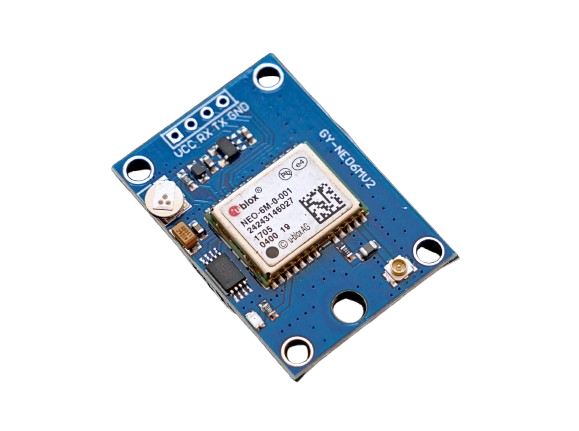
\includegraphics[scale = 0.6]{img/gps_module.png}
    \caption{Módulo GPS GY-NEO6MV2}
    \label{fig:gps_module}
\end{figure}


Algunas de sus características principales son:
\begin{itemize}
    \item Conexión UART para la comunicación con otros dispositivos, facilitando su integración con microcontroladores.
    \item Alta sensibilidad y rápido tiempo de adquisición, incluso en condiciones de baja señal.
    \item Almacenamiento de configuración mediante una memoria EEPROM interna, lo que permite guardar parámetros de configuración para su uso posterior sin necesidad de reconfigurar el módulo al encenderlo.
\end{itemize}



Gracias a su tamaño compacto y bajo consumo, el GY-NEO6MV2 es ideal para sistemas que requieren monitoreo de posición en tiempo real con un costo y consumo energético reducidos.